\chapter{Fejlesztői dokumentáció} 
\label{ch:impl}

Az alkalmazás \textbf{Microsoft Visual Studio} segítségével készült, így ha újra akarnánk fordítani akkor a \textbf{C:/} helyre csomagoljuk ki a mellékelt OGLPack.zip állományt (ez az OpenGL-hez szükséges fájlokat tartalmazza), majd futtassuk a \textbf{subst T: C:/} parancsot. Ezután megnyithatjuk a \textbf{.vcxproj} projektfájlt.

\section{Tesztelés}

A tesztelés során megvizsgáltam hogy a funkciók (\ref{sec:ui}.~fejezet) az elvártaknak megfelelően működne-e. Az ehhez használt számítógép konfiguráció:
\begin{compactitem}
	\item Intel® Core™ i7-8700 CPU
	\item 16 GB RAM
	\item NVIDIA GeForce GTX 1660 GPU
	\item Windows 10 operációs rendszer
\end{compactitem}

\subsection{Működés helyessége}

A következő viselkedéseket ellenőriztem:
\begin{compactenum}
	\item A virtuális kamerát lehet forgatni az \textbf{egérrel};
	\item A virtuális kamera nagyítását lehet állítani a \textbf{CTRL + görgővel} és a csúszkával is;
	\item A virtuális kamerát lehet mozgatni a \textbf{WASD} billentyűkkel;
	\item A mozgás sebességét lehet gyorsítani a \textbf{SHIFT} billentyűvel és álítani a görgővel vagy a csúszkával;
	\item Ha egyszerre gyorsítunk \textbf{SHIFT}-tel és görgővel, a görgő sebessége felülírja a shift gyorsítását;
	\item A fraktál paramétereit át lehet állítani a \textbf{csúszkákkal} és a fraktál ezen értékeknek megfelelően változik;
	\item A \textbf{``Zero values''} gomb hatására megközelíti minden érték a nullát;
	\item A \textbf{``Zero values''} gomb extrém érték esetén: 1000-re állítva egy csúszkát "nullázás" után az értéke 0.423 lett;
	\item A \textbf{``Random values''} gomb valóban véletlenszerű értékeket állít be. Időnként nem látható fraktálokat eredményez;
\end{compactenum}

\subsection{Teljesítmény}

Az alkalmazás erősen GPU igényes.  A futás teljesítményét az alábbi kód segítségével teszteltem:
\lstset{caption={A tesztelést végző kód}, label=src:test}
\begin{lstlisting}[language={C++}]
if (TESTING)
	{
		if (delta_time_counter < avg)
		{
			delta_time_arr[delta_time_counter] = delta_time;
			++delta_time_counter;
		}
		else
		{
			delta_time_counter = 0;
			double avg_delta_time = 0.0;
			for (int i = 0; i < avg; ++i) { avg_delta_time += delta_time_arr[i]; }
			avg_delta_time /= avg;
			printf("Avrage of delta time: %f ms   Iterations: %d   Number of spheres: %d \n", avg_delta_time*1000, iterations, ballCount);
			iterations += 2;
		}
	}
\end{lstlisting}

A kód az \textbf{Update()} függvény alján található. A \textbf{delta\_time} két képfrissítés között eltelt időt jelöli. Ezen kód segítségével \textbf{avg} darab képfrissítési idő átlagát vesszük, ezt kiírjuk az aktuális iterációk száma és mozgatható gömbök száma mellett a terminálablakra, majd ez előbbi értékét megnöveljük kettővel. A tesztek avg=100 értékkel futottak.

A tesztelés idejére ki lett kapcsolva a \textbf{vsync}, hogy ne befolyásolja a mérést. Ha be lenne kapcsolva akkor az 1/60 s = 16.66 ms-nál kisebb kirajzolási idők eredményét nem tudnánk lemérni. Továbbá az a funkció is ideiglenesen ki lett kapcsolva ami alacsony képfrissítési ráta mellett kisebbre veszi az iterációk és gömbök számát.

A kezdeti pozícióhoz képest a kamera nem volt megmozdítva, valamint a tesztben érintett két paraméteren felül más nem lett átállítva a kezdeti alapértelmezettekhez képest. A futás eredményéből készült grafikon \aref{fig:Test1}.~ábrán látható.

\begin{figure}[H]
	\centering
	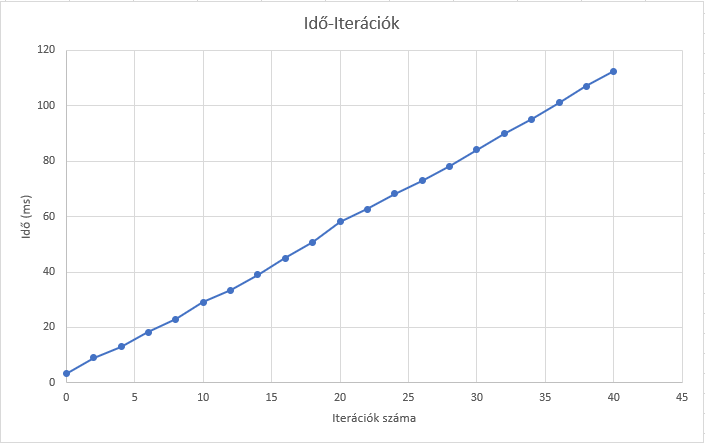
\includegraphics[width=0.8\textwidth,frame]{Test1b}
	\caption{Teljesítményteszt az iterációk számának függvényében}
	\label{fig:Test1}
\end{figure}


Megfigyelhető hogy az iterációk számától lineárisan függ a képfrissítési idő. Bármely két egymást követő sor különbsége 4-6 ms, illetve 10 iterációs eset ideje nagyjából fele a 20-nak és kb. harmada a 30-nak. Az is észrevehető hogy rettentően lelassítja az alkalmazást az iteráció növelése, elég 36-ig felmenni hogy a tesztelői környezeten 10 FPS alá essen a képfrissítési ráta (vagyis 100 ms fölé megy a frissítési idő), ami már határozattan nem folyamatos megjelenítést jelent.

Ha \aref{src:test}.~kód 15. sorát átírjuk \textbf{ballCount += 5} -re akkor azt is meg tudjuk vizsgálni hogy az mozgatható gömbök száma hogyan hat a képfrissítési időre. Ezen futás eredményéből készült grafikont \aref{fig:Test2.}~ábra mutatja.

\begin{figure}[H]
	\centering
	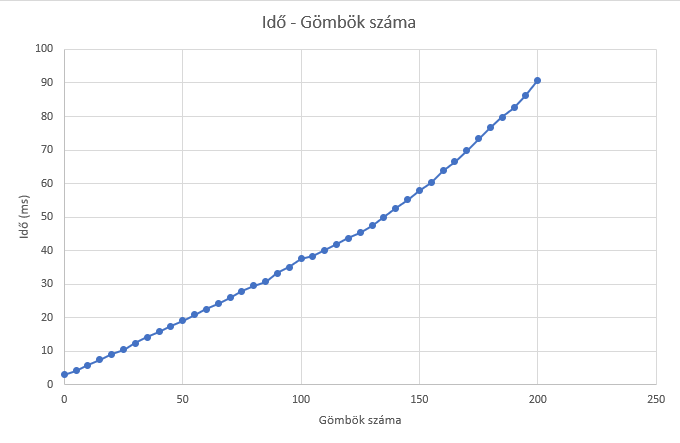
\includegraphics[width=0.8\textwidth,frame]{Test2b}
	\caption{Teljesítményteszt a gömbök számának függvényében}
	\label{fig:Test2}
\end{figure}

Itt is nagyjából lineáris összefüggést tapasztalunk, két egymás utáni érték között 1-3 ms eltérés mutatkozik, illetve az is látható hogy jóval kevesebb hatása van a gömbök számának növelése a teljesítményre. A tesztkonfigurációnak 0 iteráció mellett 40 gömb még nem okoz problémát, ellenben 0 gömb mellett 40 iteráció az előző teszt tanulsága szerint már sokkal inkább.

A gömbök esetében is inkább a megjelenítés okozza a gondot, a \textbf{glDrawArrays()} sor ideiglenes kommentezésével a kirajzolást lényegében megszüntetjük, ám az ütközések modellezését nem befolyásoljuk. Ha ezután újra futtatjuk ez előbbi tesztet, akkor megtudhatjuk hogy a fizika kiszámolása mennyire lassította a kirajzolást. A futás eredményének egy részéből készült grafikon \aref{fig:Test3}.~ábrán látható. 

A grafikonra 350-nél kevesebb gömbhöz tartozó mérési értékek nem szerepelnek, az azokhoz tartozó számolási idő kevesebb mint 1 ms volt. Ez jól mutatja hogy a kirajzolási időhöz képest az ütközések kiszámolása jelentéktelen.

\begin{figure}[H]
	\centering
	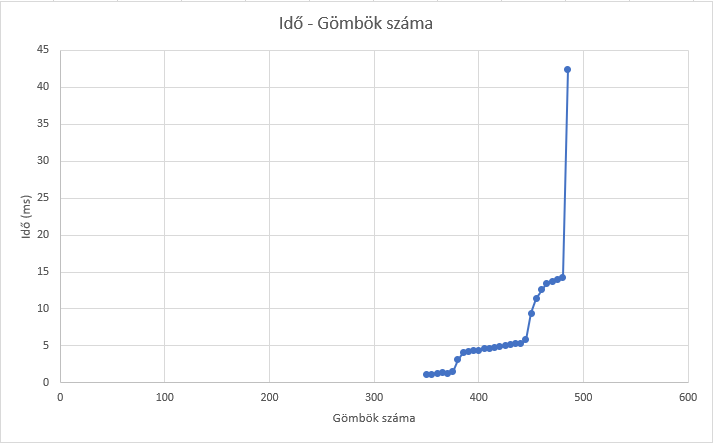
\includegraphics[width=0.8\textwidth,frame]{Test3b}
	\caption{Teljesítményteszt a gömbök számának függvényében, kirajzolás nélkül}
	\label{fig:Test3}
\end{figure}

Az ábra alapján viszont itt már inkább exponenciális összefüggést állapíthatunk meg lineáris helyett. Az utolsó érték 490 gömbbel már 1000 ms volt, de ki lett hagyva az ábrázolás megkönnyítése érdekében. A teszt alatt azonban a magasabb értékek során a processzor összesített kihasználtsága a Windows Task Manager szerint 14\%-os volt, és egyik szál sem mutatott állandó teljes terhelést.  A jelenség pontos forrása ismeretlen, de mivel csak extrém körülmények között jelentkezik, így nem lett sok idő fordítva az ok felkutatására.